\documentclass[12pt,a4paper]{article}
\usepackage[utf8]{inputenc}
\usepackage[german]{babel}
\usepackage[T1]{fontenc}
\usepackage{times}
\usepackage{graphicx}
\usepackage{url}
\usepackage{color}
\usepackage{setspace}
\usepackage{enumerate}
\usepackage{amsmath}
\usepackage{amsfonts}
\usepackage{amssymb}
\usepackage{float}
\usepackage{stix}
\title{Datenbanken}
\author{Henrik Tscherny}
\begin{document}
\maketitle
\tableofcontents

\section{Entwurf}
\paragraph{Konzeptueller Entwurf}
\begin{itemize}
\item Formale Beschreibung der Datenobjekte
\item Festlegung von Integritätsbedignungen
\item Implementierungsunabhängig
\item ER-Modell, UML-Klassenmodel
\end{itemize}
\paragraph{Logischer Entwurf}
\begin{itemize}
\item Transformation ER-Modell zu Relationsschema\\
$\rightarrow$ u.a. festlegen von Primärschlüsseln
\item Definition aktiver Komponenten
\item Vergabe von Zugriffsrechte
\end{itemize}
\paragraph{Physischer Entwurf}
\begin{itemize}
\item Umsetzung des konzeptionellen Schemas
\item Festlegung konkreter Datentypen für Attribute (int, char, ...)
\item Definition von Indexstrukturen (B-Baum / hashbasierte IS)
\item Erzeugen von Relationen
\end{itemize}
\section{ER-Modell}
\paragraph{Symbole}
\begin{table}[ht!]
\begin{tabular}{|c|c|c|}
\hline
Entität & Beziehung & Attribut\\
\hline
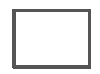
\includegraphics[scale=0.5]{./resources/enty.png} &
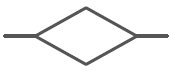
\includegraphics[scale=0.5]{./resources/rel.png} &
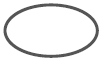
\includegraphics[scale=0.5]{./resources/attr.png} \\
\hline
\end{tabular}
\end{table}
\paragraph{Relationen}
\textbf{Funktionalitäten}
\begin{itemize}
\item 1:1
\item 1:N
\item N:1
\item N:M
\end{itemize}
\textbf{Min-Max Notation}
\begin{itemize}
(x, y)
\end{itemize}

\end{document}